
\subsection{Caja}

En este apartado se realizará un desarrollo teórico de la caja que se utilizaría para desarrollar la solución.

\subsubsection{Requisitos técnicos}

Para asegurar una protección complete de todo el sistema, se ha pensado en desarrollar una caja que mantenga protegido a todo el circuito y al sistema de carga de cualquier elemento externo que pueda perturbar su funcionamiento.

Esta protección debe asegurar las siguientes condiciones:
\begin{enumerate}
    \item \textbf{Protección contra agua y partículas}: Para evitar la entrada de agua dentro de la caja pudiendo generar cortocircuitos o dañar gravemente el funcionamiento del sistema. Estos daños también pueden ser ocasionados por la entrada de polvo u otras pequeñas partículas dentro de la caja. 
    \item \textbf{Acceso restringido}: Permitir el acceso a la carga de baterías solo se permitirá para el cliente, mientras que el acceso al circuito de carga y a la batería de backup. 
    \item \textbf{Aislamiento eléctrico}: Asegurar un aislamiento eléctrico de factores externos para evitar interferencias con el sistema.
    \item \textbf{Resistencia a golpes}: El sistema al encontrarse en un entorno al aire libre es necesario proveerlo de cierta capacidad de protección en caso de golpes o impactos de factores externos.
    \item \textbf{Resistencia rayos ultravioleta}: El sistema se carga principalmente mediante energía solar, esto implica que el sistema de carga se ve expuesto constantemente al sol y por ende a rayos ultravioleta, lo que puede dañar materiales como los polímeros.
    \item \textbf{Temperaturas de trabajo}: La caja deberá ser capaz de aguantar altas temperaturas exteriores durante largos periodos de tiempo debido al entorno al que está expuesto.
\end{enumerate}

\subsubsection{Diseño 3D}

Para tener un diseño preliminar de cómo sería la caja real se ha diseñado mediante el software de \texttt{FreeCAD} el siguiente modelo en 3D:

\begin{figure}[H]
    \centering
    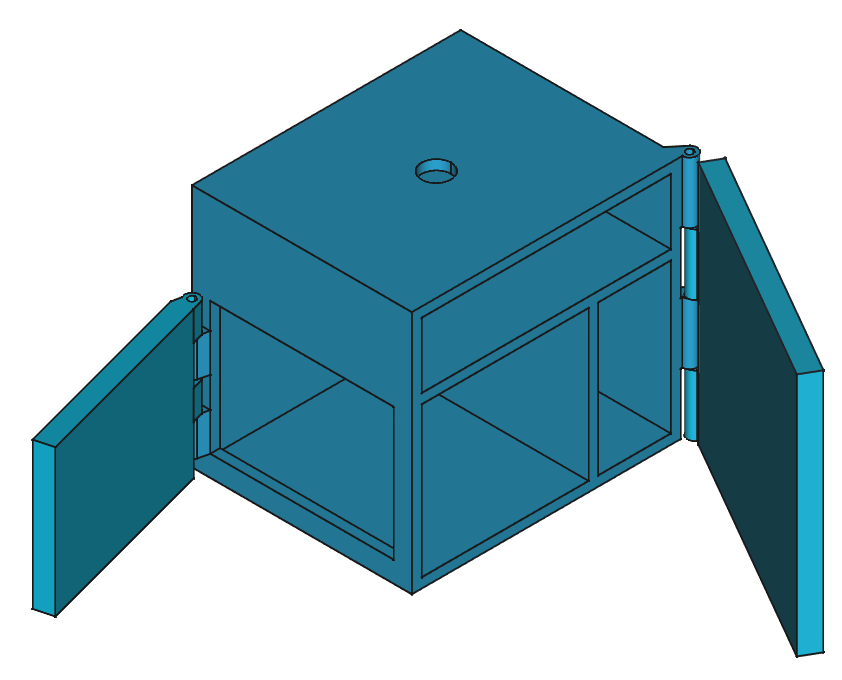
\includegraphics[width=0.45\textwidth]{images/4-DesarrolloTeorico/4-1-caja/CAJA_3D_ISOMETRICA.png}
    \caption{Vista Isométrica Modelo 3D caja}
    \label{fig:DesarrolloTeorico/Caja/CAJA_3D_ISOMETRICA}
\end{figure}

Como se puede observar, la caja cuenta con 2 accesos:
\begin{itemize}
    \item \textbf{Puerta de usuario}: Esta puerta es usada por el cliente para únicamente conectar/desconectar las baterías que se desean cargar.

\begin{figure}[H]
    \centering
    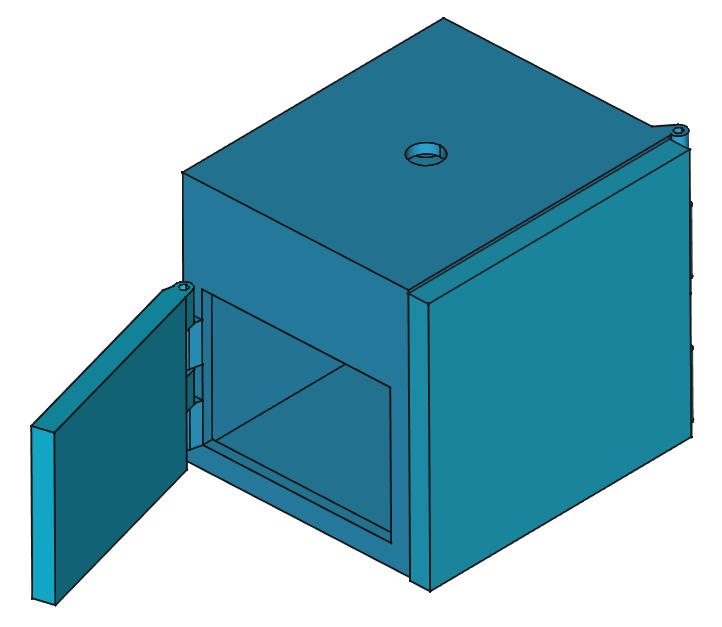
\includegraphics[width=0.35\textwidth]{images/4-DesarrolloTeorico/4-1-caja/CAJA_3D_PUERTA_USER.png}
    \caption{Vista Puerta Usuario Modelo 3D caja}
    \label{fig:DesarrolloTeorico/Caja/CAJA_3D_PUERTA_USER}
\end{figure}

    \item \textbf{Puerta de técnico}: Esta puerta es usada por el personal de administración para acceder tanto al circuito de carga como las baterías de backup y que estén cargándose.
\begin{figure}[H]
    \centering
    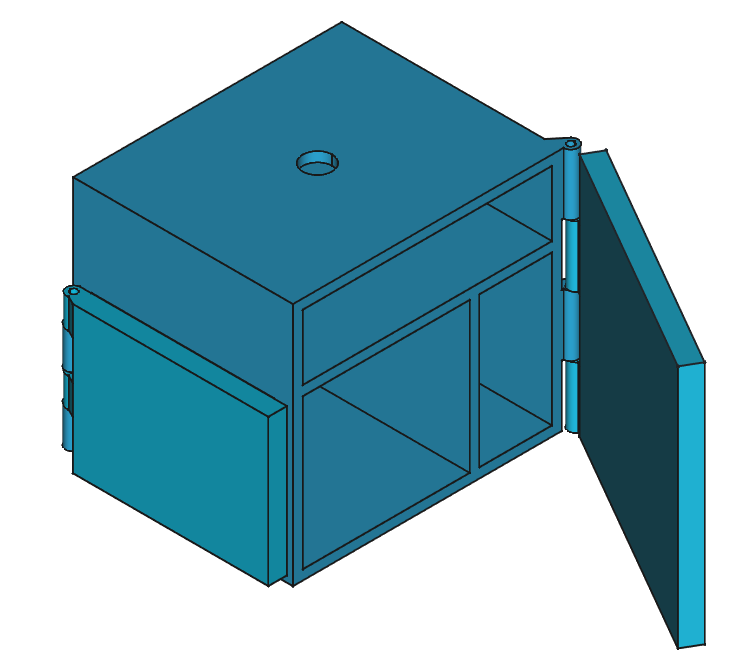
\includegraphics[width=0.35\textwidth]{images/4-DesarrolloTeorico/4-1-caja/CAJA_3D_PUERTA_ADMIN.png}
    \caption{Vista Puerta Técnico Modelo 3D caja}
    \label{fig:DesarrolloTeorico/Caja/CAJA_3D_PUERTA_ADMIN}
\end{figure}

\end{itemize}

Adicionalmente, el interior de la caja tiene 3 incisiones. Estas serán usadas únicamente para dar acceso a los terminales de carga para las baterías del usuario (los 2 accesos de la izquierda) y la de backup (acceso de la derecha).

\begin{figure}[H]
    \centering
    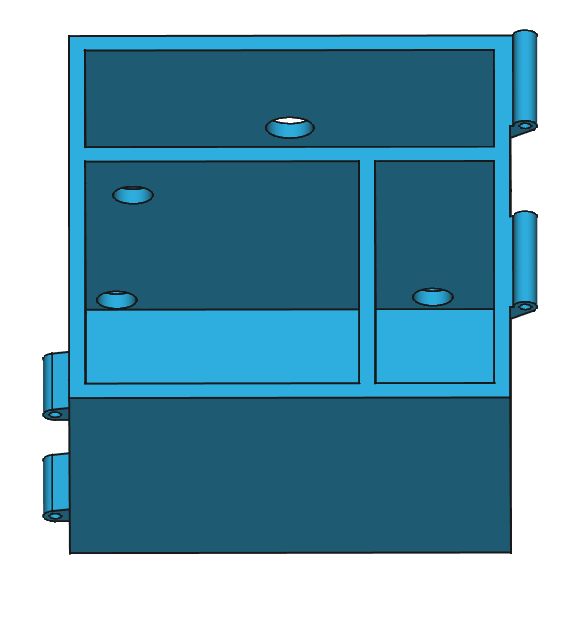
\includegraphics[width=0.35\textwidth]{images/4-DesarrolloTeorico/4-1-caja/CAJA_3D_ACCESOS.png}
    \caption{Vista Incisiones Modelo 3D caja}
    \label{fig:DesarrolloTeorico/Caja/CAJA_3D_ACCESOS}
\end{figure}


Además, en la parte superior de la caja contamos con un acceso para la entrada del cableado del panel solar para la caja.

\textbf{Nota}: Para facilitar el entendimiento del diseño en el \autoref{sec:anexo_caja} se encuentran en detalle todas las vistas del diseño sin las puertas e imágenes adicionales del mismo.

\subsubsection{Características técnicas}

Para cumplir el diseño teórico se proponen las siguientes características técnicas:
\begin{itemize}
    \item \textbf{Protección contra agua y partículas:} La caja cumplirá la norma internacional CEI 60529 para permitir esta protección. En concreto una protección IP67 que garantiza una protección completa contra polvo y pequeñas partículas y además, la inmersión completa de la caja a sin filtración alguna. \cite{iecInternationalStandardIEC}

    \item Acceso restringido: Esto se logra con el diseño 3D que hemos propuesto para la caja, la única implementación adicional que es necesaria añadir son cerraduras en cada una de las puertas.

    \item \textbf{Aislamiento eléctrico, resistencia rayos ultravioleta y temperatura:} Para esto se plantea que el material de la caja sea de policarbonato. Gracias a esto se consigue evitar el efecto de jaula de Faraday que pudiera causar el uso de una caja de metal. Además, el policarbonato proporciona una protección total de los rayos ultravioleta y una temperatura de operación desde \texttt{-40ºC} hasta \texttt{115ºC} siendo un rango más que de sobra para nuestro circuito. \cite{horeshPolycarbonateProtectionUV2021} Además, protege de posibles cortos en caso de que alguno de los elementos de la caja hiciera contacto con ella.

    Como elemento adicional, todo el cableado expuesto tanto en el interior de la caja (cableado usado por el usuario) como exteriores (cableado del panel solar) pasarán por prensaestopas y el cableado exterior constará de una funda de protección para el paso del panel a la caja.
    \begin{figure}[H]
        \centering
        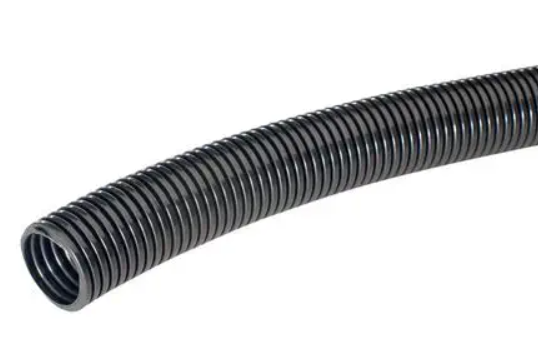
\includegraphics[width=0.4\textwidth]{images/4-DesarrolloTeorico/4-1-caja/CAJA_FUNDAS.png}
        \caption{Funda cableado exterior}
        \label{fig:DesarrolloTeorico/Caja/CAJA_FUNDA}
    \end{figure}

    \begin{figure}[H]
        \centering
        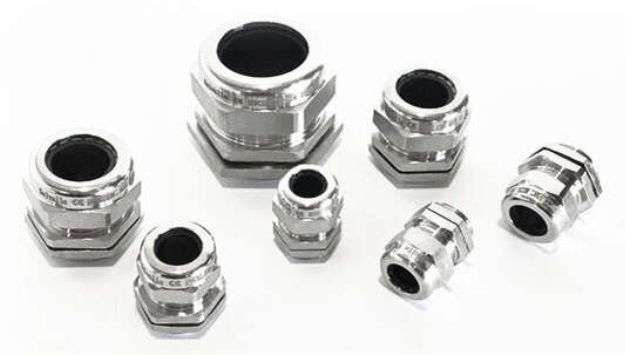
\includegraphics[width=0.4\textwidth]{images/4-DesarrolloTeorico/4-1-caja/CAJA_PRENSAESTOPAS.png}
        \caption{Prensaestopa}
        \label{fig:DesarrolloTeorico/Caja/CAJA_PRENSAESTOPA}
    \end{figure}


    \item \textbf{Resistencia a golpes:} En caso de impactos la caja debe proporcionar cierta protección, para esto debe de asegurar un índice de protección \texttt{IK} entre $08$ y $09$ que ayudaría a mitigar los golpes de efectos adversos como el granizo o golpes de pequeñas rocas. \cite{iecInternationalStandardIEC}

\end{itemize}